% AE646 Stage 3 final presentation - Team PINNacles
% Build:  tectonic FINAL_PRESENTATION.tex   ->  FINAL_PRESENTATION.pdf
% (the submitted copy is docs/PINNacles_Stage3_FinalPresentation.pdf)
\documentclass[aspectratio=169,11pt]{beamer}

\usetheme{Madrid}
\usecolortheme{whale}
\setbeamertemplate{navigation symbols}{}
\setbeamertemplate{caption}{\raggedright\insertcaption\par}
\usepackage{booktabs}
\usepackage{amsmath,amssymb}

\title[FNO for Parametric Darcy Flow]{Operator Learning for Parametric Darcy Flow}
\subtitle{Fourier Neural Operator vs.\ MLP Baseline --- Stage 3}
\author[Team PINNacles]{Team PINNacles \\ \small Aryamann Srivastava}
\institute[IIT Kanpur]{AE646: Scientific Machine Learning for Fluid Mechanics \\ Department of Aerospace Engineering, IIT Kanpur}
\date{November 2026}

\begin{document}

\begin{frame}\titlepage\end{frame}

\begin{frame}{Problem}
\begin{columns}
\begin{column}{0.56\textwidth}
2D parametric Darcy flow (steady pressure in a porous medium):
\[ -\nabla\cdot(\kappa(x,y)\,\nabla u(x,y)) = f,\quad (x,y)\in(0,1)^2 \]
\[ u = 0 \text{ on } \partial\Omega,\qquad f = 1 \]
\begin{itemize}
  \item $\kappa\in\{0.1,1.0\}$: piecewise-constant permeability (thresholded Gaussian random field).
  \item Goal: learn the solution operator $\mathcal{G}:\kappa \mapsto u$ once, then evaluate in milliseconds.
\end{itemize}
\end{column}
\begin{column}{0.42\textwidth}
\footnotesize
\textbf{Why it matters.} Classical solvers (FDM/FEM) re-solve the full PDE for every new $\kappa$; UQ / optimisation / control need thousands of solves.
\medskip

\textbf{Theme \#8}: operator learning for parametric PDEs. Baseline = MLP; SciML model = FNO.
\end{column}
\end{columns}
\end{frame}

\begin{frame}{Dataset --- real PDEBench 2D Darcy ($\beta=1.0$)}
\begin{itemize}
  \item Official source: DaRUS / Uni Stuttgart, DOI \texttt{10.18419/darus-2986}; checksum-verified download (\texttt{src/download\_data.py}). 10\,000 samples at native $128\times128$.
  \item Reproducible (seed 42), non-overlapping subset: \textbf{900 train / 100 validation / 200 test} --- matching the sample counts used by Li et al.\ (2021).
  \item Main pipeline at $64\times64$: subsample every second grid point. Normalisation uses training statistics only.
  \item The 200 test samples are \emph{also} kept at native $128\times128$ (\texttt{test\_hires.npz}) --- untouched real ground truth for the zero-shot super-resolution check.
\end{itemize}
\end{frame}

\begin{frame}{Models}
\begin{columns}
\begin{column}{0.5\textwidth}
\textbf{MLP baseline}
\begin{itemize}\footnotesize
  \item Flatten $64{\times}64{\times}3 \to 3{\times}2048$ (GELU) $\to 64{\times}64$.
  \item 42.0\,M parameters. No spatial inductive bias; input size hard-locked to $64\times64$.
\end{itemize}
\end{column}
\begin{column}{0.5\textwidth}
\textbf{Fourier Neural Operator}
\begin{itemize}\footnotesize
  \item Lift $3\to64$; $4\times$ [SpectralConv (12 modes) $+$ $1\times1$ conv $+$ LayerNorm $+$ GELU]; project $64\to128\to1$.
  \item Spectral weights live in Fourier space $\Rightarrow$ resolution-invariant.
  \item Original: 4.7\,M params. Improved: width 128, 20 modes, 6 blocks $\Rightarrow$ 78.8\,M.
\end{itemize}
\end{column}
\end{columns}
\vfill
\footnotesize Training: Adam ($10^{-3}$, cosine to $10^{-5}$), batch 16, weight decay $10^{-4}$, relative-$L_2$ loss. 100 epochs (200 for FNO improved); the lowest-validation-error checkpoint is kept (no early stopping). Metric reported in physical (denormalised) units.
\end{frame}

\begin{frame}{Test-set accuracy ($64\times64$, 200 held-out samples)}
\centering
\begin{table}
\begin{tabular}{lrrrrrr}
\toprule
Model & Params & Mean & Median & Std & Min & Max \\
\midrule
MLP baseline & 42.0\,M & 0.0820 & 0.0695 & 0.0456 & 0.0325 & 0.3367 \\
FNO original &  4.7\,M & 0.0521 & 0.0398 & 0.0451 & 0.0155 & 0.3467 \\
FNO improved & 78.8\,M & \textbf{0.0456} & \textbf{0.0307} & 0.0487 & \textbf{0.0106} & 0.3535 \\
\bottomrule
\end{tabular}
\end{table}
\vfill
\begin{itemize}\footnotesize
  \item FNO original: \textbf{37\% lower mean error than MLP with $9\times$ fewer parameters}.
  \item Scaling to 78.8\,M ($17\times$) buys only a further 12\% --- the 12-mode truncation, not channel count, is the limit.
  \item Similar std across models ($0.045$--$0.049$): the hard cases (complex multi-region $\kappa$) are hard for every architecture.
\end{itemize}
\end{frame}

\begin{frame}{Error distribution and parameter efficiency}
\begin{columns}
\begin{column}{0.58\textwidth}
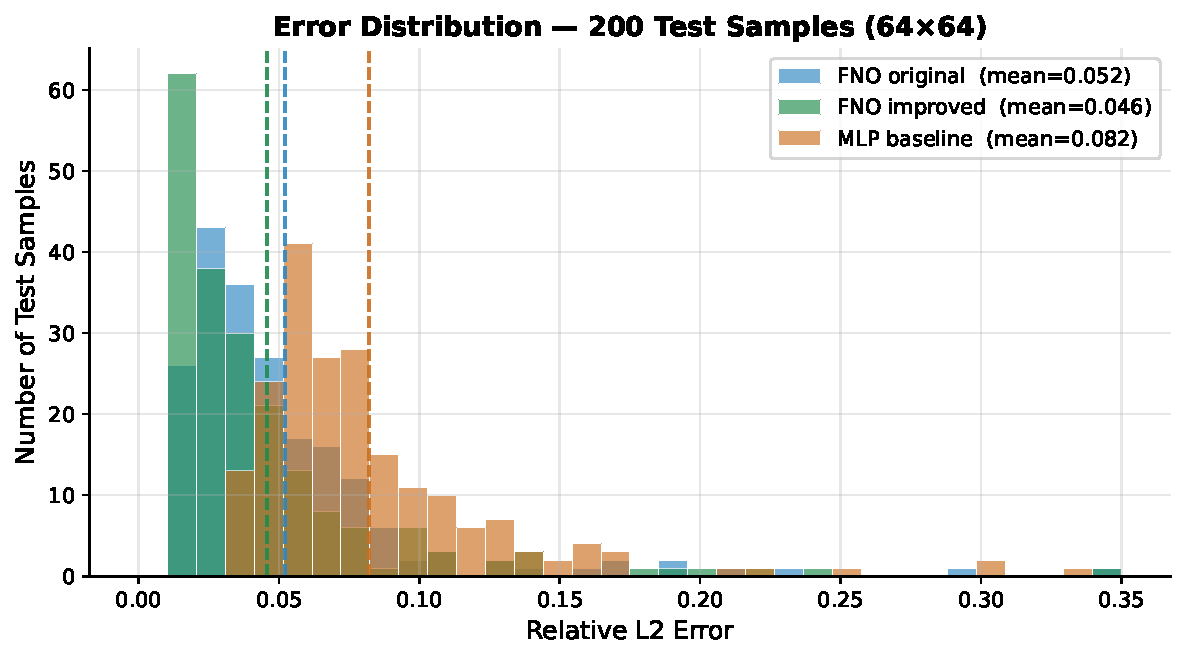
\includegraphics[width=\linewidth]{../results/figures/fig1_error_histogram.pdf}
\end{column}
\begin{column}{0.42\textwidth}
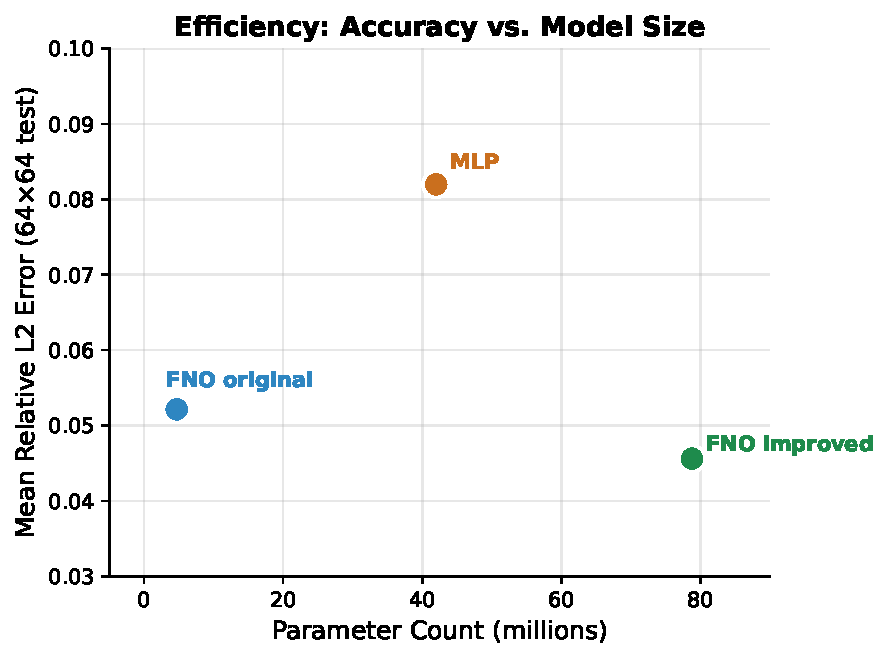
\includegraphics[width=\linewidth]{../results/figures/fig2_efficiency_scatter.pdf}
\end{column}
\end{columns}
\vfill
\footnotesize Right-skewed errors: most samples well below 0.1, a $\lesssim5\%$ tail with highly heterogeneous $\kappa$ drives the maximum toward 0.35. FNO sits in the favourable low-parameter / low-error corner.
\end{frame}

\begin{frame}{Zero-shot super-resolution (evaluate at native $128\times128$)}
\begin{columns}
\begin{column}{0.5\textwidth}
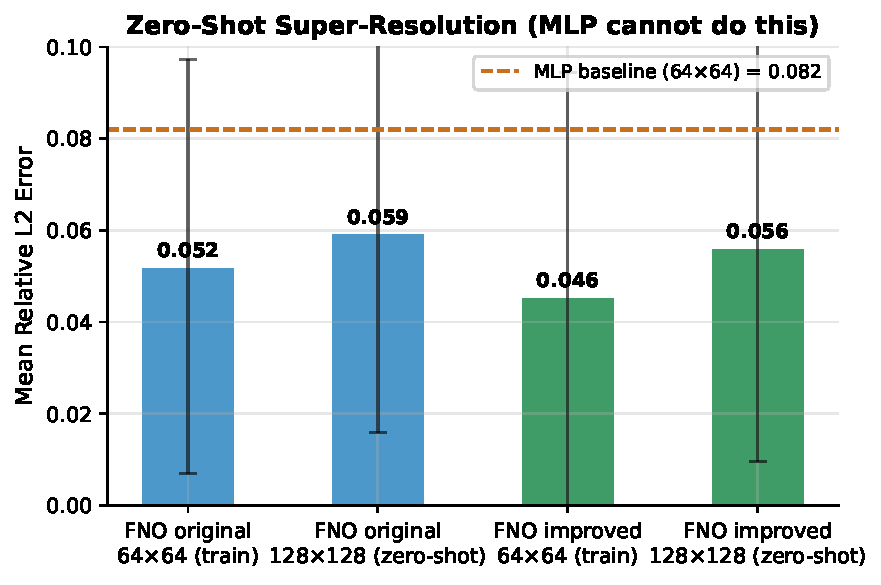
\includegraphics[width=\linewidth]{../results/figures/fig3_superres.pdf}
\end{column}
\begin{column}{0.5\textwidth}
\footnotesize
\begin{table}
\begin{tabular}{lrr}
\toprule
Model & $64^2$ (train) & $128^2$ (zero-shot) \\
\midrule
FNO original & 0.0521 & 0.0594 \\
FNO improved & 0.0456 & 0.0563 \\
\bottomrule
\end{tabular}
\end{table}
\medskip
Same weights, real native-resolution $\kappa$, \emph{no} retraining. Error rises only $+14\%$ (original): Darcy solutions are low-frequency dominated, so the unmodelled high modes carry little energy. The MLP cannot run this test at all (fixed input size).
\end{column}
\end{columns}
\end{frame}

\begin{frame}{Inference speed}
\begin{columns}
\begin{column}{0.52\textwidth}
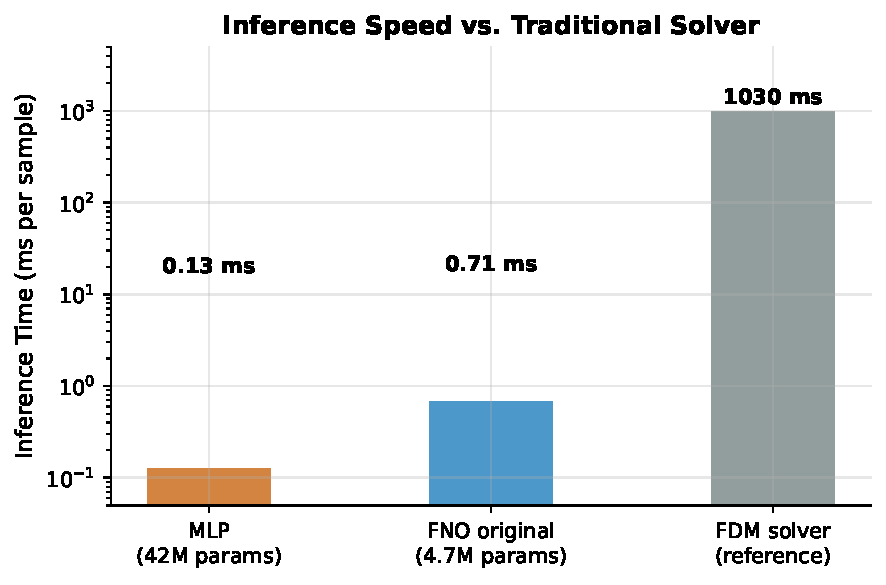
\includegraphics[width=\linewidth]{../results/figures/fig4_speed.pdf}
\end{column}
\begin{column}{0.48\textwidth}
\footnotesize
\begin{table}
\begin{tabular}{lrr}
\toprule
Solver & ms/sample & vs.\ FDM \\
\midrule
FDM (SciPy sparse, CPU) & 1030.1 & $1\times$ \\
MLP baseline (GPU) & 0.13 & $7740\times$ \\
FNO original (GPU) & 0.71 & $1443\times$ \\
\bottomrule
\end{tabular}
\end{table}
\medskip
Both surrogates are $>1000\times$ faster than the numerical solver. MLP is $\sim5.4\times$ faster than FNO per sample (FFT latency) --- but FNO's accuracy makes it the better operator surrogate.
\end{column}
\end{columns}
\end{frame}

\begin{frame}{Where does FNO spend its time?}
\begin{columns}
\begin{column}{0.55\textwidth}
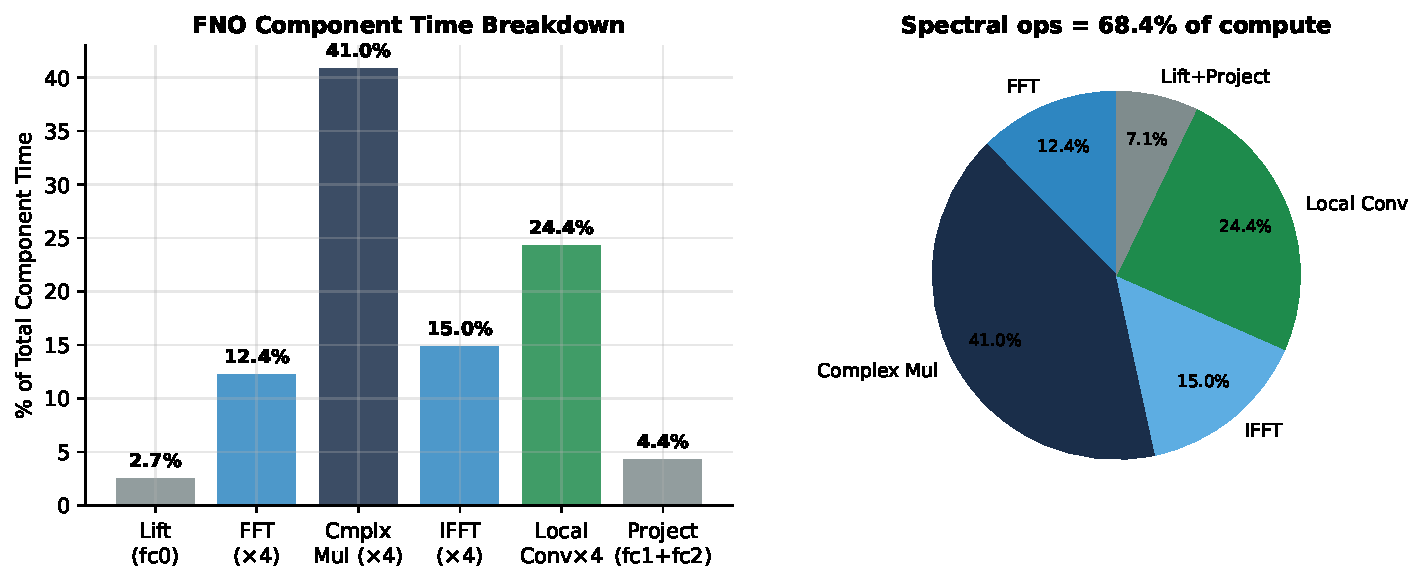
\includegraphics[width=\linewidth]{../results/figures/fig5_components.pdf}
\end{column}
\begin{column}{0.45\textwidth}
\footnotesize
Layer-wise profiling with a device sync before every timer read (measured on Apple Silicon / MPS, 500 iterations).
\begin{itemize}
  \item Spectral ops (FFT $+$ complex multiply $+$ IFFT): \textbf{68.4\%}.
  \item Complex weight multiply alone: \textbf{41.0\%} --- a batched einsum over $64{\times}64{\times}12{\times}12$ complex tensors.
\end{itemize}
Sync-per-timer inflates absolute times ($\approx$19.6\,ms) far above the fused 0.71\,ms; the \emph{relative} split is the portable result. Optimisation target: low-rank / Tucker-decomposed spectral weights.
\end{column}
\end{columns}
\end{frame}

\begin{frame}{Physical interpretation}
\begin{itemize}
  \item Darcy pressure $u$ solves an elliptic PDE: globally smooth, low-wavenumber dominated. FNO's 12-mode truncation \emph{is} this prior --- it keeps the coefficients that carry the energy.
  \item MLP flattening destroys locality in the first layer; its 42\,M-parameter map is poorly regularised for the task and must learn spatial correlations by brute force.
  \item High-error samples ($\epsilon > 0.2$): many disconnected $\kappa$ regions with sharp interfaces $\Rightarrow$ rapid transitions in $\nabla u$ needing high modes. Adding modes/depth helps the easy and typical cases (median $0.0398 \to 0.0307$) but barely moves the worst case ($0.347$ vs.\ $0.354$).
\end{itemize}
\end{frame}

\begin{frame}{Conclusion and reproducibility}
\begin{itemize}
  \item FNO beats the MLP baseline: \textbf{37\% lower error, $9\times$ fewer parameters}, zero-shot to $2\times$ resolution ($+14\%$), $>1000\times$ faster than FDM.
  \item The spectral inductive bias --- ``elliptic PDE solutions are smooth'' --- is nearly exact for Darcy flow, which explains the gap with the unbiased MLP.
  \item Reproducible: seed 42 throughout; \texttt{pytest} suite (16 tests); metrics/figures regenerate from committed JSON; MPS re-run of the pipeline matched the GPU numbers (FNO 0.0521 vs.\ 0.0544).
\end{itemize}
\vfill
\footnotesize \textbf{AI-tool declaration.} Claude Code assisted with debugging (the GPU timing fix), LaTeX formatting, and slide-build scripting. All results are from experiments run on real hardware; every number, figure, and claim was reviewed and is owned by the author. Full statement: \texttt{CONTRIBUTION\_STATEMENT.pdf}.
\end{frame}

\begin{frame}{References}
\footnotesize
\begin{enumerate}
  \item Z.\ Li et al., ``Fourier Neural Operator for Parametric Partial Differential Equations,'' ICLR 2021.
  \item M.\ Takamoto et al., ``PDEBench: An Extensive Benchmark for Scientific Machine Learning,'' NeurIPS 2022. DOI \texttt{10.18419/darus-2986}.
  \item N.\ Kovachki et al., ``Neural Operator: Learning Maps Between Function Spaces,'' JMLR 2023.
\end{enumerate}
\vfill
\centering Thank you --- questions welcome.
\end{frame}

\end{document}
